\documentclass{article}
\usepackage{ctex}
\usepackage{amsmath}
\usepackage{graphicx}
\usepackage{wrapfig}
\usepackage{caption}
\usepackage[top=0.8in, bottom=0.8in,left=0.8in, right=0.8in]{geometry}
\usepackage{float} 
\usepackage{subfigure}
\usepackage{subcaption}
\usepackage{bm}
\xeCJKsetup{CJKmath=true} 
\title{\textbf{第二届$\Sigma Pho$物理竞赛}\\试题部分}
\date{2023年12月}
\begin{document}
\maketitle
\begin{flushright}
    命题:胡锦浩、盛铖开、应佑、李骏亭、孙可名\\
	审题:胡锦浩、盛铖开、应佑、李骏亭、孙可名\\
    组题:胡锦浩\\
\end{flushright}
$$\textbf{考生必读}$$
\begin{itemize}
\item[1.]\textbf{考生考试前请务必阅读本须知。}
\item[2.]\textbf{本试题共 8 题,满分 320 分。}
\item[3.]\textbf{如遇到试题印刷不清楚的情况,请向监考老师提出。}
\item[4.]\textbf{需要阅卷老师评阅的内容一定要写在答题纸相应题号后面的空白处;阅卷老师只评阅答题纸上的内容,写在试题纸和草稿纸上的内容一律不被评阅。}
\end{itemize}
\section*{第一题、功亏一篑(40分)}
众所周知,台球先打彩球,最后打黑8,但若打黑8时白球同时进洞,则直接判对方获胜。小s同学就经常干这类愚蠢之事,现建模分析。\par
若已知每个球的质量为$m$,重力加速度为$g$,桌面滑动摩擦系数为$\mu$,半径为$R$。
\begin{itemize}
\item[(1)]求打击何处时,可以使其直接进入纯滚。(杆对球的力沿水平方向)
\item[(2)]若小s同学用(1)方式击打白球,使其获得速度$v_0$,撞击与洞口距离为$l$的黑8(弹性正碰,且白球,黑8,洞口共线,忽略两球间摩擦)。
\begin{itemize}
\item[(2.1)]白球是否会进洞?
\item[(2.2)]求白球在入洞前摩擦力做的功。
\item[(2.3)]若白球进洞,求白球在黑球之后多久入洞。若白球不进洞,求白球停在距洞多远处。
\end{itemize}
\end{itemize}
\section*{第二题、打飞机奇遇I(40分)}
小s同学一天看到天上飞过一架漂亮国的飞机,于是想设计一个电磁炮把它打下,现在来分析这一过程。
\begin{itemize}
\item[(1)]小s同学先设计了一个可以产生$\vec{B}=k\cdot z^{3/2}\hat{z}$磁感应强度的线圈,然后以$v_0$从$z=0$(以炮弹尾而言)处发射一枚炮身电导率为$\sigma$的金属圆柱壳,其厚度为$t$,弹头为绝缘材料的炮弹,已知炮管长$L$,不计重力,求出射时炮弹速度。炮身长$l$,半径为$r$,炮弹总质量为$m$.
\item[(2)]但是小s同学惊奇的发现(1)中的炮弹出射速度小于$v_0$,于是他重新进行设计,仅将电导率为$\sigma$的金属壳换成超导圆柱壳,初始磁通量为零,磁感应强度改为$\vec{B}=(B_0-kz)\hat{z}$,其他参量均不变,且$B_0>k(L+\frac{l}{2})$将炮弹从$z=0$处(相对弹尾而言)静止释放,不记重力,求出射速度。
\item[(3)]设计完成后他还不满足,又设计了一新型炮弹,全部为绝缘材料,但体心有一微小的,通有恒流$I$,半径为$R$的金属环(可视为磁偶极子)磁场改为$\vec{B}=k\cdot z^{\alpha}\hat{z}$,炮弹质量为$m$,炮身长$L$,初始时位于$z=0$(相对金属环而言)处,求出射速度。
\end{itemize}

\section*{第三题、物质电导的经典理论(40分)}
经典电子论的基础是由P.K.L.Drude在1900左右提出的。其模型如下:
\begin{itemize}
\item[1.]将金属分为固定不动(可在附近做振动)的原子核和自由移动的电子(自由电子气,满足能均分定理)。
\item[2.]自由电子的运动决定了金属的导热性与导电性。
\item[3.]自由电子与原子核碰撞来交换能量,从而达到热平衡。
\end{itemize}
\begin{itemize}
\item[(1)]Ohm定律,简单认为电子以平均速率$\bar{u}$运动,且与原子核相碰后完全失去定向移动速率,设平均自由程为$\bar{\lambda}$,电子热运动以热运动平均速率$\bar{u}$运动。\par
试证明:
\[
\vec{j}=\sigma\vec{E}
\]
并给出$\sigma$,用电子质量$m$,电量绝对值$e$,数密度$n$(一价金属),平均自由程$\bar{\lambda}$表示。
\item[(2)]Joule-Lenz定律,电子与原子核相碰后,其动能完全转化为原子核的热振动动能,给出热运动功率密度(单位体积内放出的热能)。用电场$\vec{E}$与一个用上已知量表示的常数给出。
\item[(3)]Wiedemann-Frantz定律,给出导热系数$\kappa$的微观表达式以及与电导率$\sigma$之间的关系
\end{itemize}
\par
提示:傅里叶热传导定律
\[
j_q=-\kappa\dfrac{\mathrm{d}T}{\mathrm{d}z}
\]\par
其中$j_q$为单位时间流过单位面积的能量。\par
注意:本题无需考虑Maxwell速率分布
\section*{第四题、打飞机奇遇II(40分)}
经过巨长时间,小s同学终于造好了电磁炮,准备开始打飞机了。
\begin{itemize}
\item[(1)]小s同学想先检验自己的力量,于是先用手扔炮弹,已知此速度下空气阻力为$\vec{f}=-k\vec{v}=-m\beta\vec{v}$,小s同学抛出炮弹的速度为$v_0$,与竖着方向夹角为$\theta_0$,质量为$m$,重力加速度为$g$,以抛出点为原点,求$x(t),y(t)$
\item[(2)]没上过几节体育课的小s同学力量不够,炮弹打不到飞机,于是他启用了新建的电磁炮,在此速度下阻力近似为$\vec{f}=-m\beta|\vec{v}|\vec{v}=-c|\vec{v}|\vec{v}$,已知初速度为$v_0$,\textbf{角度为$\theta_0$(与上题不同,此为与水平方向夹角)},重力加速度为$g$,质量为$m$。
\begin{itemize}
\item[(2.1)]列出自然坐标系下的动力学方程(可带曲率半径$\rho$)
\item[(2.2)]以$v,\theta$为变量列出微分方程并积分得$v(\theta)$,并得到炮弹最高点的速度,再代入 $\beta =0$检验你的结果.\par
提示:用$\rho$的自然坐标表示式,并用$v\cos\theta$换元.\par
    \[
    \int \dfrac{\mathrm{d}\theta}{\cos^3\theta}=\dfrac{1}{2}\left(\dfrac{\sin\theta}{\cos^2\theta}+\ln\dfrac{1+\sin\theta}{\cos\theta}\right)
    \]
\item[(2.3)]若用电磁炮直接轰击漂亮国的首都,(不考虑地球弯曲),且出射速度极大$\theta_0=0$轨道近似为直线,在此条件下求解$x$关于$t$的函数,并求出轨迹方程$y(x)$ (提示:用$\rho$的直角坐标表示)
\end{itemize}
\end{itemize}
\section*{第五题、简单热力学(40分)}
本题探究热力学方程得出热力学参量。\par
补充:Maxwell关系
$$
\begin{aligned}
\left( \dfrac{\partial T}{\partial V}\right) _{S}=-\left( \dfrac{\partial p}{\partial S}\right) _{V}\\
\left( \dfrac{\partial T}{\partial p}\right) _{S}=+\left( \dfrac{\partial V}{\partial S}\right) _{p}\\
\left( \dfrac{\partial S}{\partial V}\right) _{T}=+\left( \dfrac{\partial p}{\partial T}\right) _{V}\\
\left( \dfrac{\partial S}{\partial p}\right) _{T}=-\left( \dfrac{\partial V}{\partial T}\right) _{p}\\
\end{aligned}
$$
\begin{itemize}
    \item[(1)]对于气体系统
    \begin{itemize}
        \item[(1.1)]试证:$$\left(\dfrac{\partial U}{\partial V}\right)_T=-p+T \left(\dfrac{\partial p}{\partial T}\right)_V$$
        \item[(1.2)]试证:对于任意系统,均有$$\left(\dfrac{\partial C_V}{\partial V} \right)_T=T\left(\dfrac{\partial^2 p}{\partial T^2}\right)_V$$
        \item[(1.3)]给出$1\ \mathrm{mol}$气体的Van der Waals方程$$\left(p+\dfrac{a}{V^2}\right)(V-b)=RT$$\par
        试证明其定容摩尔热容仅是温度的函数,并在温度变化不大时,求出其内能与熵的表达式,可含积分常数。
        \item[(1.4)]Redlich-Kwong方程考虑了温度及密度对分子间作用力的影响.\par
        $1\mathrm{mol}$的R-K方程为$$p=\dfrac{RT}{V-b}-\dfrac{a}{\sqrt{T} V(V+b)}$$
        给定$V\to 0$时,其定容摩尔热容$C_{V_0}(T)$.试求任意状态时其$C_V$的值.
    \end{itemize}
    \item[(2)] 对于表面系统,给定表面的张力系数$\sigma(T)$.液体表面积用$A$表示
    \begin{itemize}
        \item[(2.1)] 已知自由能$F=U-TS$是求表面系统的内能与自由能的微分表达式.\par 提示:需要考虑温度的影响
        \item[(2.2)] 在等温条件下,对$F$进行积分.求出$F$的表达式.(积分常量由自己定需符合实际)
        \item[(2.3)] 前两问进行对比得出表面系统熵和内能的表达式.
    \end{itemize}
\end{itemize}
\section*{第六题、虚光子与作用力(40分)}
近代物理认为,粒子之间碰撞时的能量变化是通过交换粒子完成的,本题对此种物理过程作一些简单的计算与分析(\textbf{送分题,不要跳过——出题人})
\begin{itemize}
    \item[(1)] 试就两粒子以任意大小、方向的动量发生碰撞,证明此过程若是为两粒之间传递一个粒子,该粒子的质量不可能为非零实数。(仅就正碰情况下讨论的不得分)
    \item[(2)] 在该类过程中较短时间$\Delta t$内,交换的粒子允许的能量守恒的微小偏离$\Delta E$,若满足Heisenberg不确定关系,即$\Delta E\cdot \Delta t\le\dfrac{\hbar}{2}$此问取$\Delta E\cdot \Delta t\ \~{}\ \hbar$,作用力程为$\Delta r$,试估计交换粒子的静能,用$\Delta r$与若干常数表示。
    \item[(3)] 对于核力,其力程约为$\Delta x\approx 2\mathrm{fm} $试估计核力中交换粒子的静能.
    \item[(4)] 基于此种思想,Y.Yukawa通过核力与电磁力的类比提出核力的介子理论.认为核力的作用是通过交换$\pi$介子完成的,$\pi$介子的存在于12年后得到证实。\par 该粒子分为$\pi^0,\pi^+,\pi^-$分别带电$0,e,-e$,质子中子利用其产生作用的方式,如下图\par
    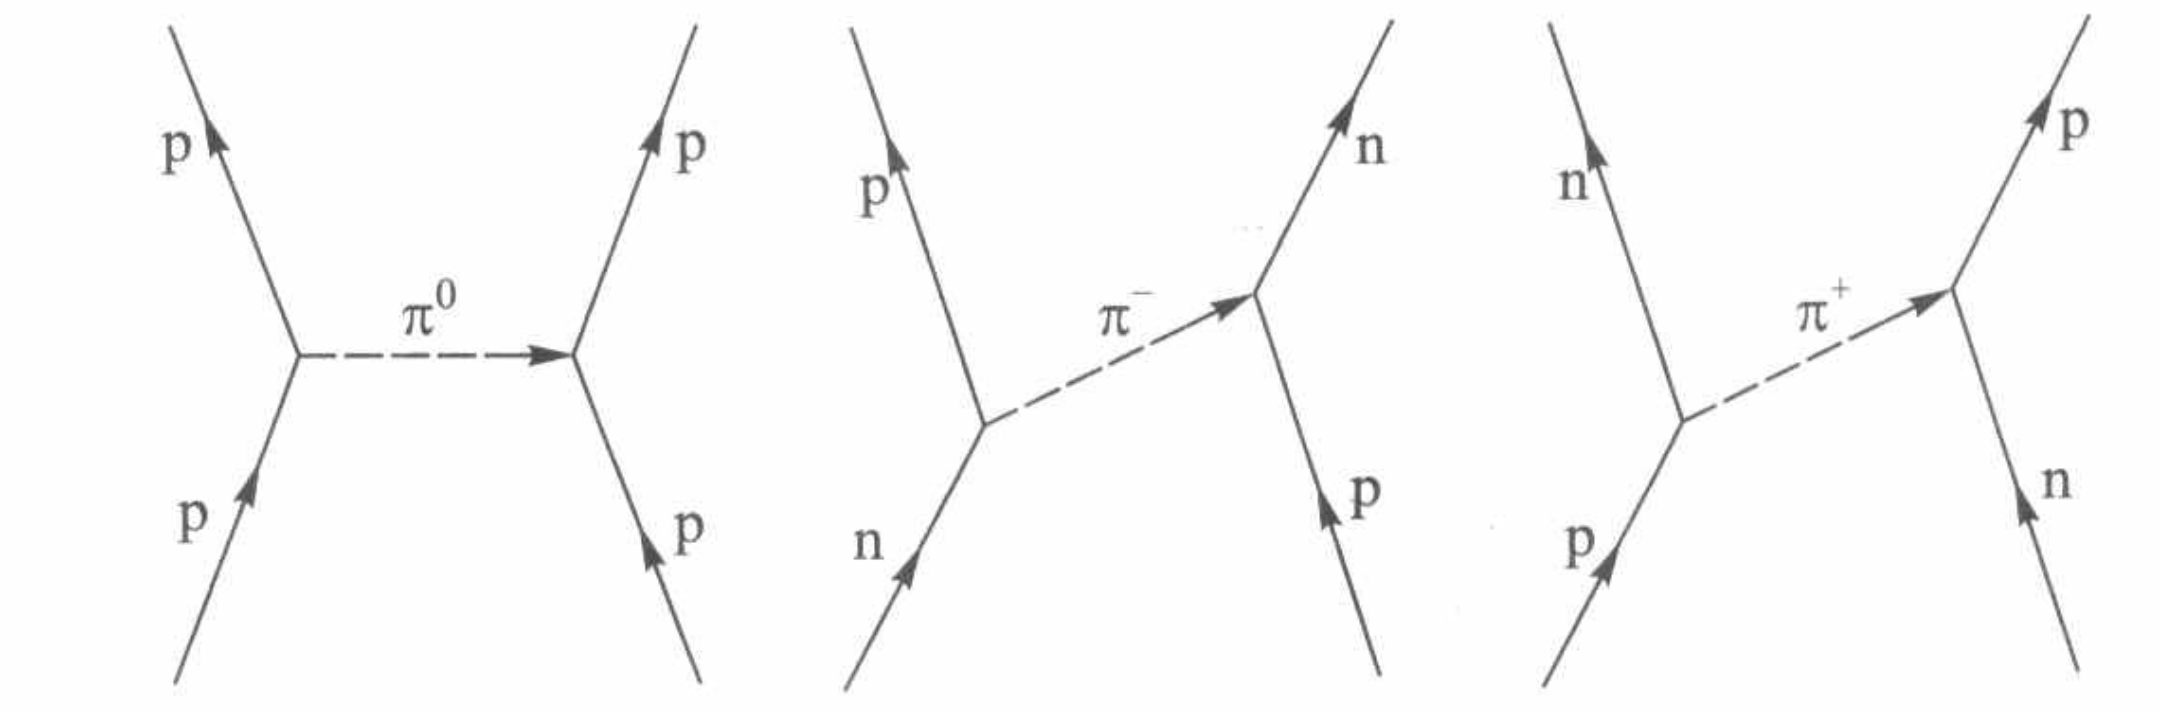
\includegraphics[scale=0.4]{img/0012.1.png}\par
    并在以上过程可保持初末粒子几乎静止,已知$|m_p-m_n|\ll m_{\pi}$.粒子波函数为复数形式的球面波(与光波相同),试证明$\pi$介子的动量为虚数并给出核子间相互作用势能(与波函数成正比)与$r$的依赖关系.
    \item[(5)] 请回答电磁相互作用中交换粒子是?
\end{itemize}
\clearpage
\section*{第七题、Kerr盒(40分)}
\begin{wrapfigure}{r}{5cm}
	\vspace{-15pt}    % 对应高度1
	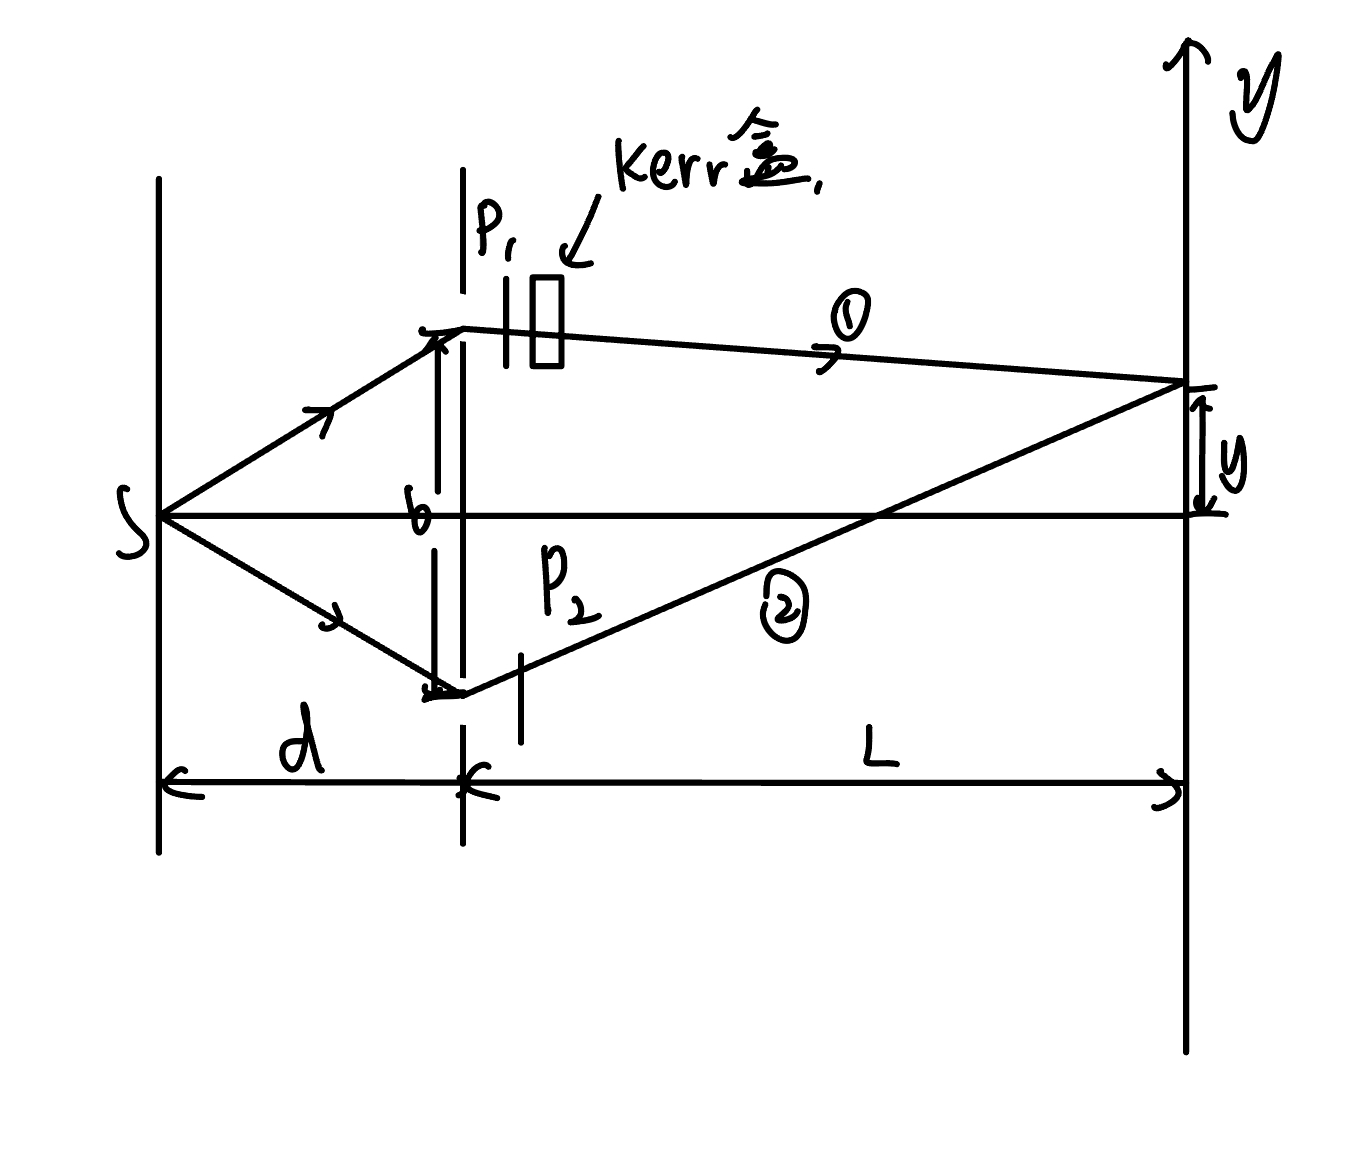
\includegraphics[width=5cm]{img/0013.1.jpeg}\\
	\vspace{-15pt}    % 对应高度2
	\caption{}
	\vspace{-15pt}    % 对应高度3
\end{wrapfigure}
 已知Kerr盒相当于一波晶体片,因其导致o光,e光间光程差满足下式$$\dfrac{\Delta}{2\pi}=\dfrac{|n_o-n_e|d}{2\pi}=B\dfrac{E^2 d}{\lambda}$$其中$d$为Kerr盒长。\par
如图偏振片$P_1, P_2$偏振方向夹角为$\theta$,$o$振动光矢量垂直于主平面.
Kerr盒对应光轴方向垂直于$P_2$偏振方向,双缝干涉参数如图。
\begin{itemize}
    \item[(1)] 试求光线$\textcircled{1}$通过Kerr盒后椭圆偏振光的椭圆参数.即长轴大小,方向(用通过偏振片后振幅$A$表示)
    \item[(2)] 试求屏上光强分布$$T(y)=\dfrac{1}{T}\int^T_0|\vec{E}|^2\mathrm{d} t$$
    \item[(3)] 试求衬比度$$\gamma=\dfrac{I_{max}-I_{min}}{I_{max}+I_{min}}$$
\end{itemize}
\section*{第八题、可爱的杆(40分)}
\begin{wrapfigure}{r}{5cm}
	\vspace{-15pt}    % 对应高度1
	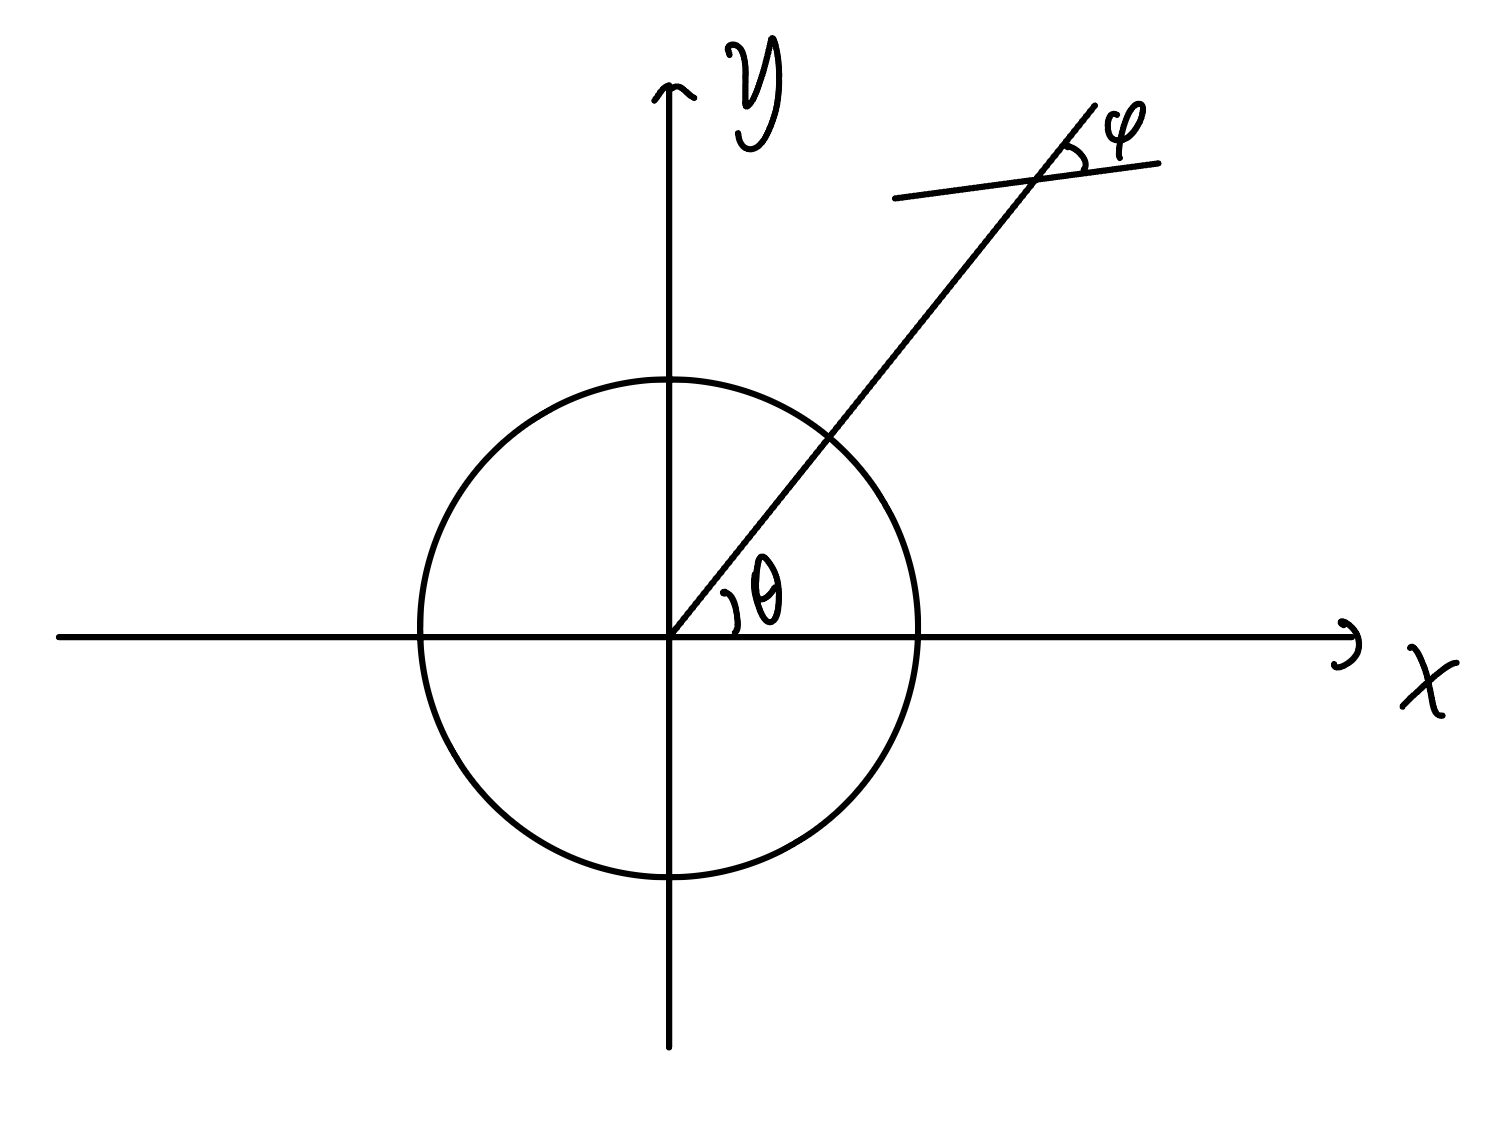
\includegraphics[width=5cm]{img/0010.1.jpeg}\\
	\vspace{-15pt}    % 对应高度2
	\caption{}
	\vspace{-15pt}    % 对应高度3
\end{wrapfigure}
一根杆位于太空中绕一质量为$M$的中心天体旋转。杆质地坚硬,长为$2l$,质量为$m$,杆质心距离中心天体$r$,角度$\varphi$如图所示,已知$r\gg l$
\begin{itemize}
\item[(1)]求使$r,\dot{\theta},\varphi$不随时间变化的\textbf{稳定的}$\varphi$值。并求出此时$r,\dot{\theta}$应满足的关系,保留至 $\frac{l^2}{r^2}$阶。
\item[(2)]
\begin{itemize}
    \item[(i)]设系统原来以(1)中稳定的运动方式运动,现给杆微扰,使其具有一定的$\dot{r},\dot{\varphi}$初始值,试求有关$r,\theta,\varphi$的运动微分方程
    \item[(ii)]令$r=r_0+\Delta r$,$\dot{\theta}=\omega_0+\Delta \omega$,其中满足$\dfrac{\Delta r}{r_0}\ \~{}\ \dfrac{\Delta \omega}{\omega_0} \ \~{}\ \varphi\ \~{}\ \dfrac{l^2}{l_0^2}\ll 1$,试求$\varphi$可以具有的两种频率(不必求出特解),并判断两频率是否与$l$相关。试就两频率的来源分别简述原因
    \item[(iii)]  求此时杆质心运动的旋进角速度(进动角速度)。(原运动完成一个周期后,矢径转过的角度与原运动得到周期比值)
\end{itemize} 
\end{itemize}
\end{document} 